\section{Bayesian Trust Framework}
To assess our trust in the other peers in the system, we implemented
the model from ``B-trust: Bayesian Trust Framework for Pervasive Computing''
\cite{btrust}. The paper describes a method of maintaining context-sensitive
information about previous direct experiences with other peers as well as
the recommended trust received from third-party recommenders. Trust values
are stored probabilistically and trust evolution from one
experience/recommendation to another uses a form a Bayes' theorem.

\subsection{Rationale}
This paper was chosen for implementation because: it's data structures scale
linearly with respect to the number of peers tracked; and it embodies what
id describes as three main properties of trust, subjectiveness,
context-dependence, and dynamism. These three properties explained are:
\begin{itemize}
  \item Subjectiveness: identical actions taken by different agent may lead to
  different levels of trust;
  \item Context-dependence: trust in one context does not necessarily transfer
  to another; and
  \item Dynamism: ``trust increases after successful observations, while it
  decays over time''~\cite{btrust}.
\end{itemize}

The same behavior may lead to
different trust lev- els in different trusting entities, hence subjectiveness
qualifies trust. As trust (e.g., in giving good advices) in one context (e.g.,
academia) does not necessarily transfer to an- other context (e.g., industry), we
add context-dependence to the list of trust properties. Finally, the fact that
trust increases after successful observations, while it decays over time
exemplifies its dynamism. As a result, trust evolution must embed the notion of
time.



\subsection{Theory}
For each context and peer, we store a vector that represents a discrete
probability mass function (pmf) of our direct trust $d_\alpha$, which is the
trust formed from previous direct experiences with this peer. We similarly store a
vector for the recommended trust pmf $r_\alpha$, which is the trust formed from
recommendations received about this peer from third-parties.

Again for each context and peer, we store two matrices (direct and recommended)
which govern the evolution of trust. By scaling the feedback when the trust
pmfs evolve, these matrices control how much the pmfs change when we receive
additional information about a peer. In terms of Bayes' theorem, the
values in these matrices are conditional probabilities which act as weights
to the prior probabilities of the trust level.

These pmfs are initialized to the uniform discrete distribution, which
represents a lack of information about this peer's behaviour. After a few rounds
of trust evolution, the mean $\mu_{\{d,r\}}$ of this pmf \eqref{eq:bayes_mean}
is a single value representing our direct/recommended trust in a given peer,
while the variance $\sigma^2_{\{d,r\}}$ of the pmf \eqref{eq:bayes_variance}
represents our confidence in this trust value. The uniform discrete distribution
has the highest variance $\sigma^2_U = \frac{n^2-1}{12}$, while the degenerate
distribution has the lowest $\sigma^2_\delta = 0$, so we map this variance range
into a confidence value on [0,1] using \eqref{eq:bayes_confidence}.

\begin{equation}
\label{eq:bayes_mean}
\mu_{\{d,r\}} = \sum_{i=0}^{n-1}{i*{\{d,r\}}_i}
\end{equation}

\begin{equation}
\label{eq:bayes_variance}
\sigma^2_{\{d,r\}} = \sum_{i=0}^{n-1}{i^2*{\{d,r\}}_i} - \mu^2_{\{d,r\}}
\end{equation}

\begin{equation}
\label{eq:bayes_confidence}
c = 1 - \frac{\sigma^2_{\{d,r\}}}{\sigma^2_U}
\end{equation}


\subsection{Implementation}

\begin{figure}[h!]
  \centering
  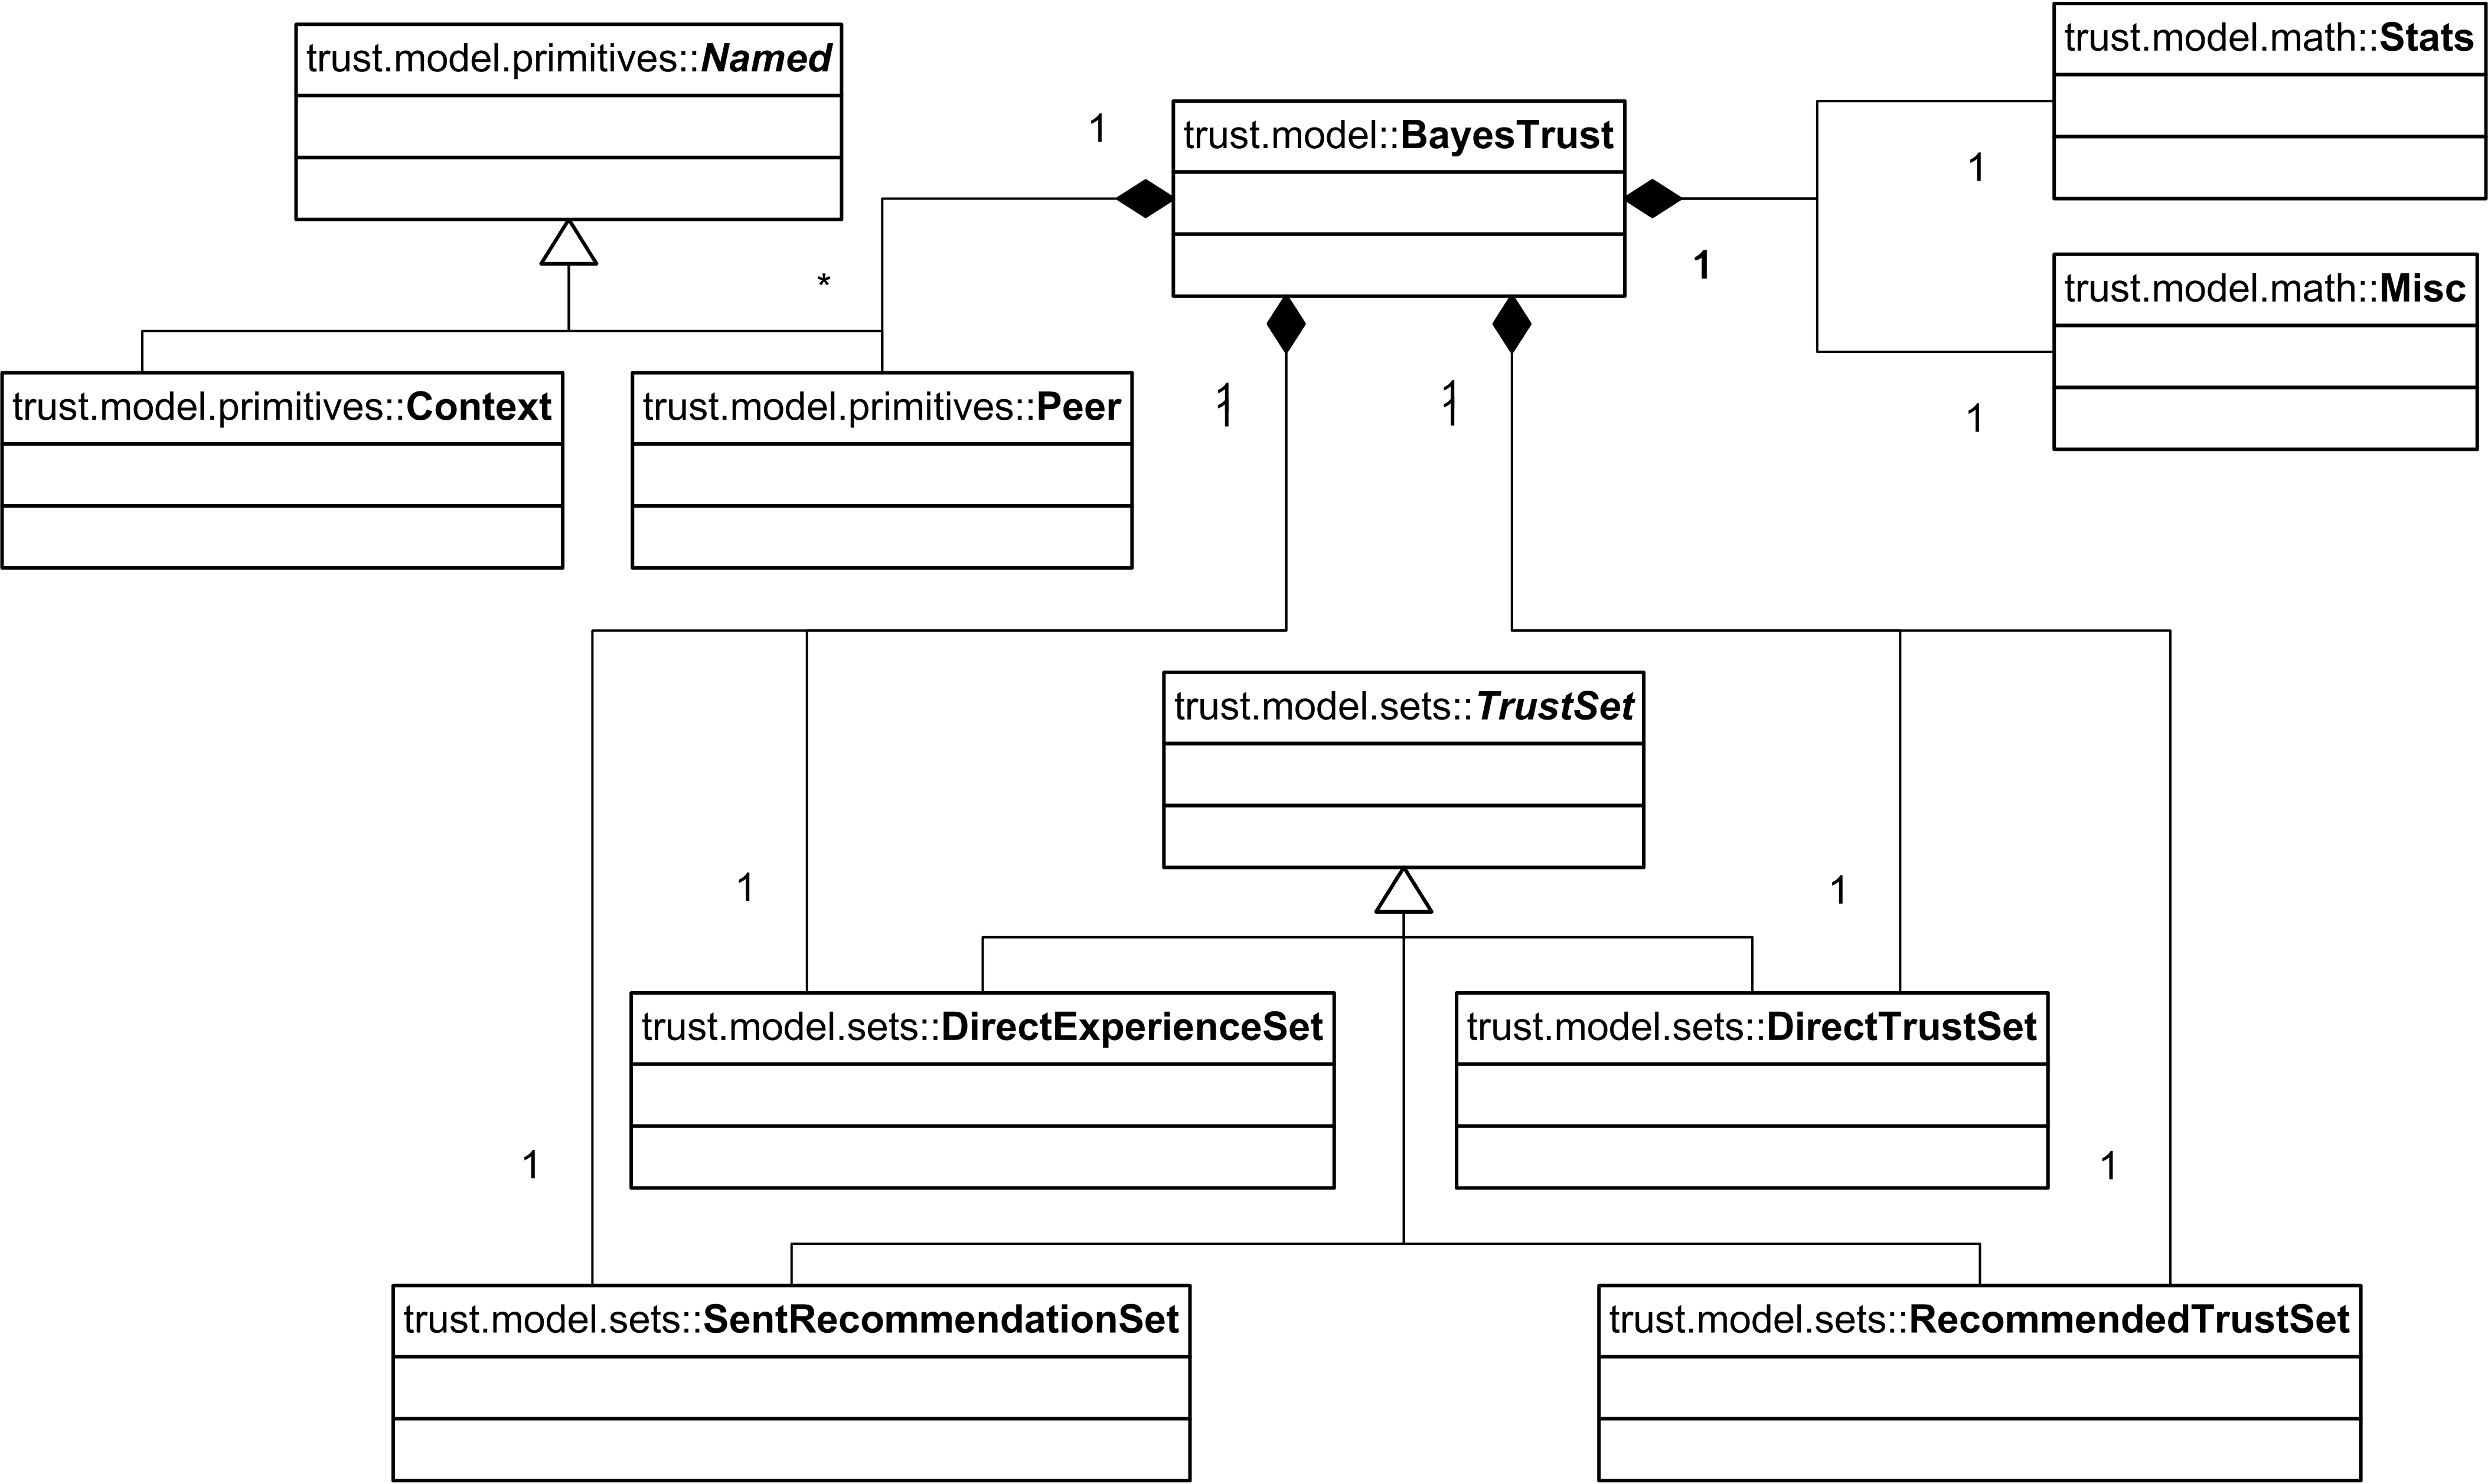
\includegraphics[width=1\textwidth]{images/bayestrust}
  \caption{Bayes Trust Framework High Level Class Diagram}
  \label{fig:xml2dttest}
\end{figure}

\begin{figure}[h!]
  \centering  
  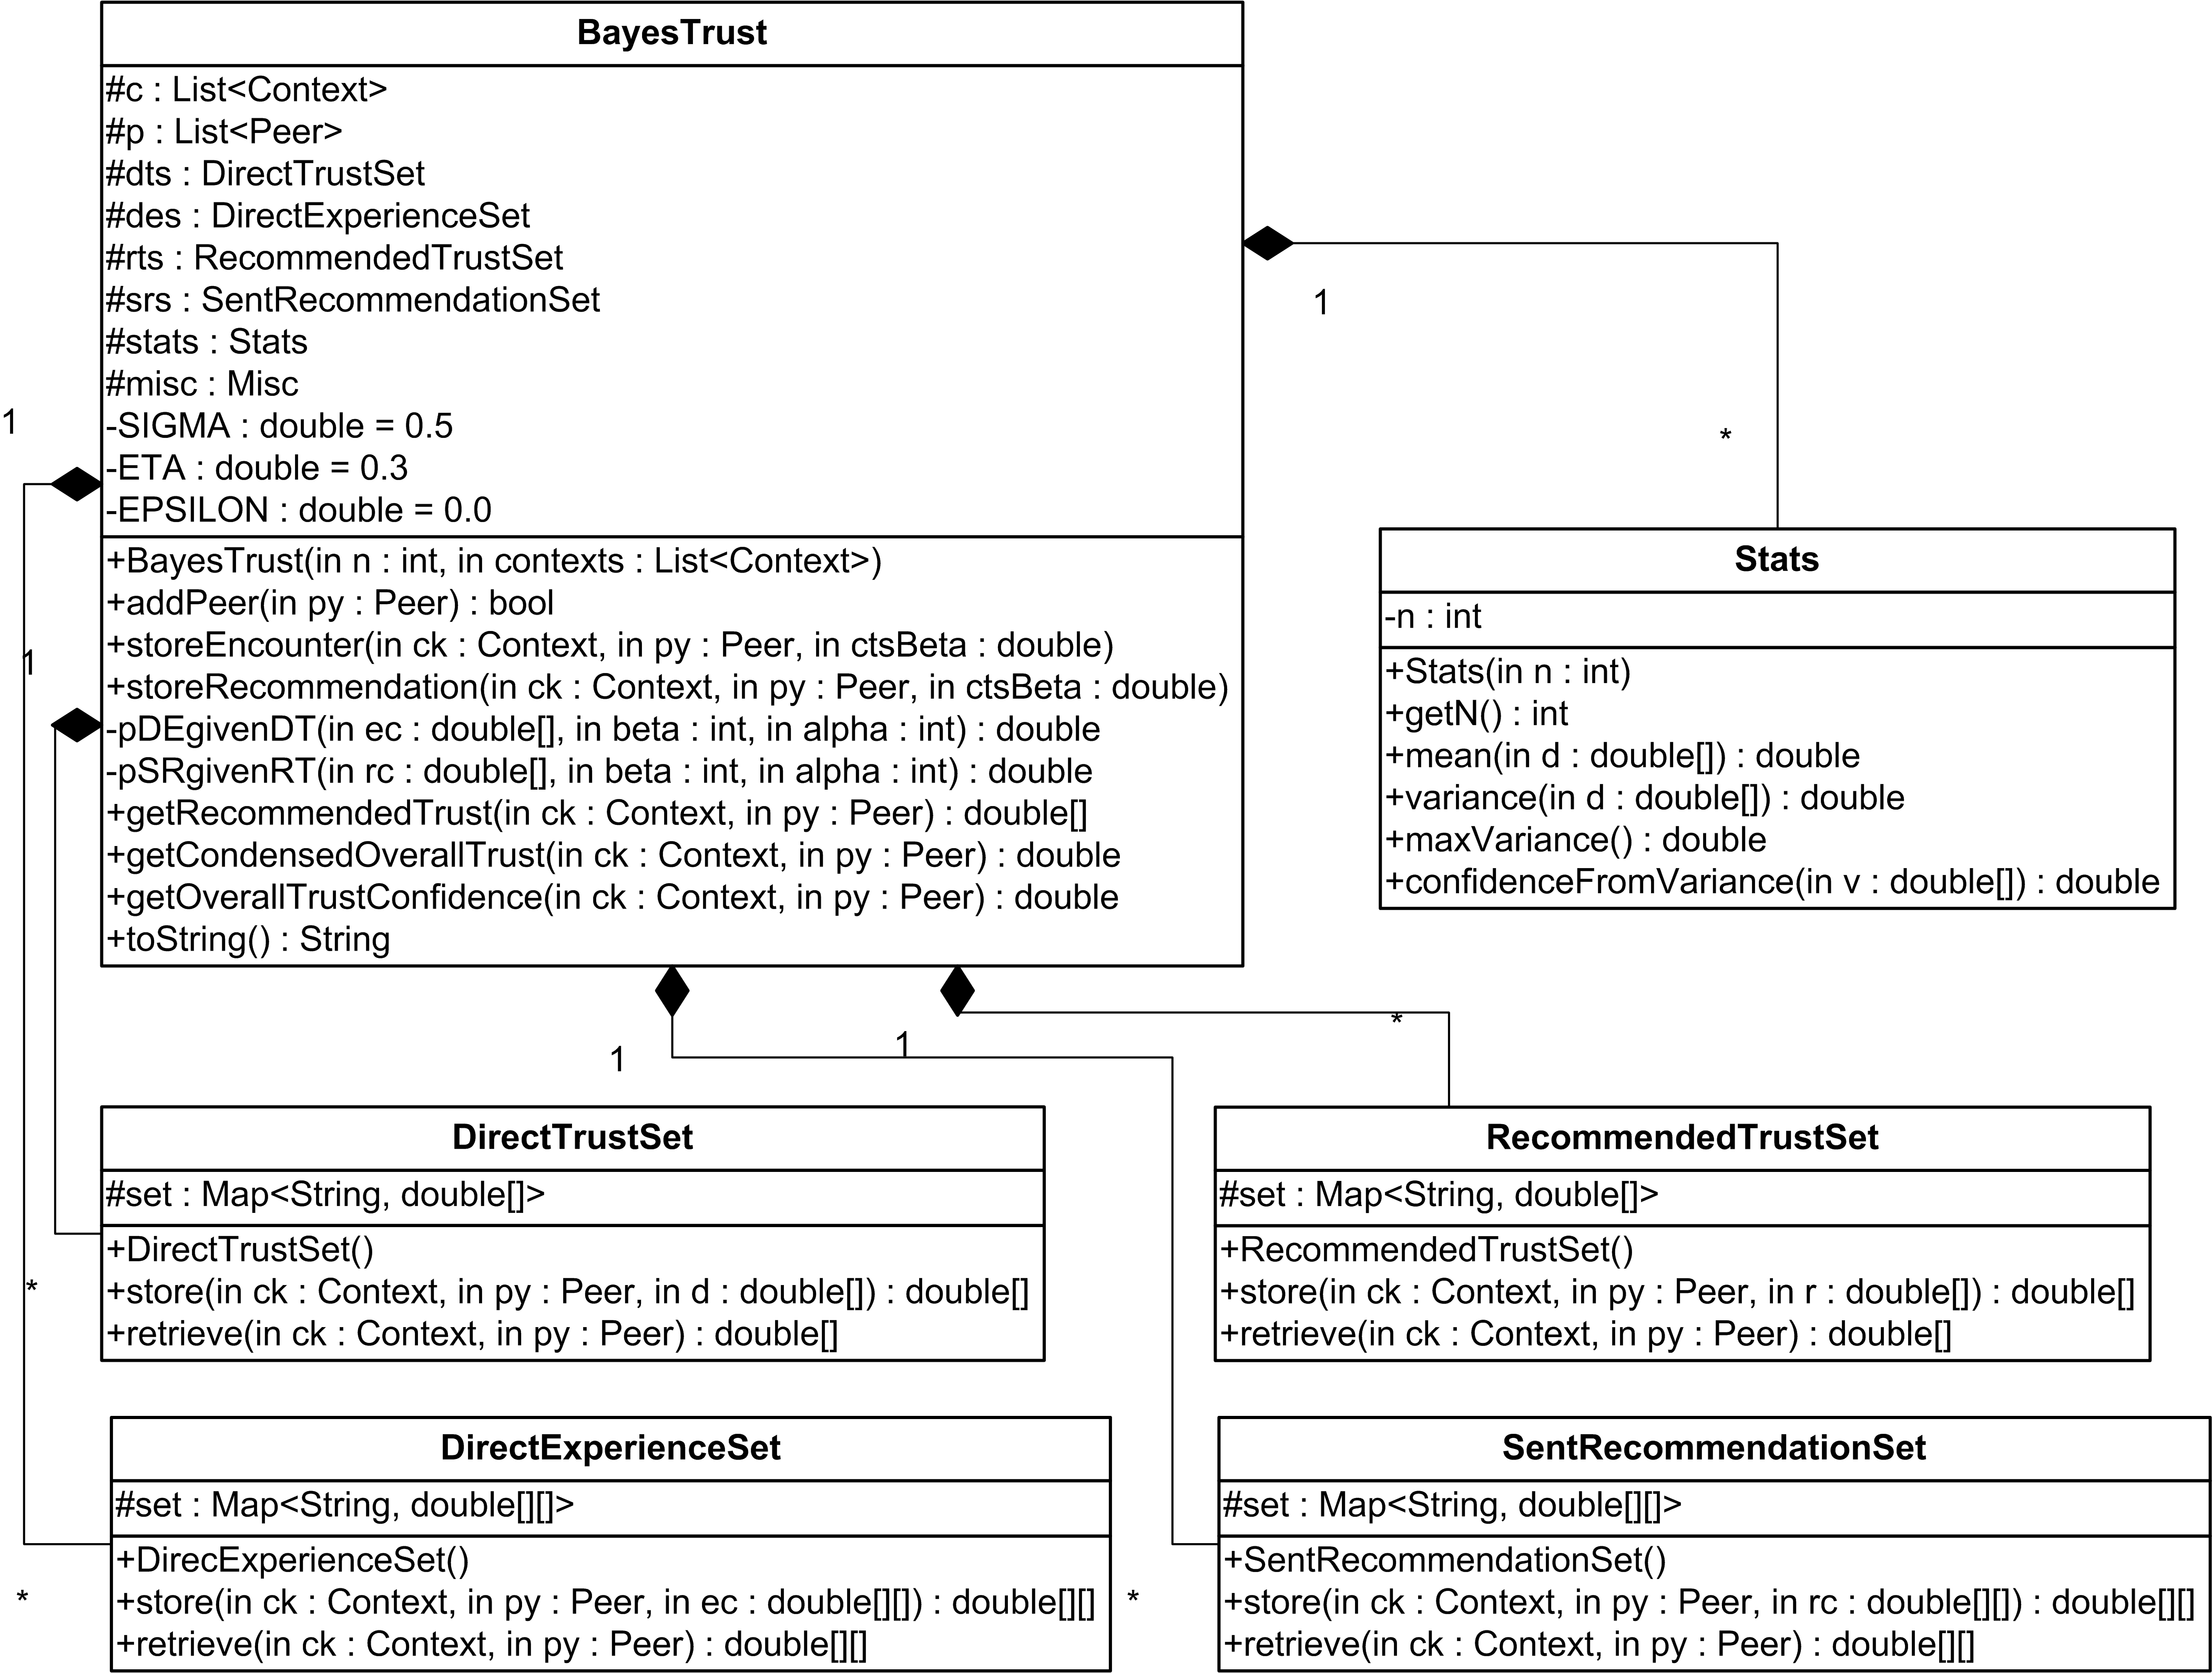
\includegraphics[width=1\textwidth]{images/bayestrustdetail}
  \caption{Bayes Trust Framework Detailed Class Diagram}
  \label{fig:xml2dttest}
\end{figure}


\subsection{Testing}
Unit tests for the framework